\chapter{The Dynamics of Molecular Liquids}
\label{sec:dynamics}

The motion of a molecule is comprised of two components, the translational motion described by movements of the center of mass, and rotational motion described by changes in the orientation of the molecule. In a liquid, both translational and rotational motions will involve cooperative motion with the neighbouring molecules. The nature of the cooperation is different for each type of motion. Translational motion requires a vacant space to move into often giving rise to string like sequences of molecular translations~\tocite. Rotational motion is more dependent on the shape of the molecule, a molecule that approximates a circle is going to be able to rotate more easily than an elongated rod. 

In this Chapter we want to investigate the influence of molecular shape on the coupling of the rotational and translational motions as well as the role of molecular shape in the overall dynamics. To begin we must introduce some model molecules a choice we describe in \textsecref{mol choice}. Next, we shall introduce the various dynamic quantities we will be using to characterise the motion of the molecules in the liquid state \secref{dynamic quantities}. In the subsequent Sections we present our analysis of the dynamics of our model molecules.


\section{Choice of Molecules}
\label{sec:mol choice}

Our goal in studying these molecular systems is not to reproduce the behaviour of a specific molecule, but rather to explore how basic features of all molecules, namely shape, influence the molecular motion in the liquid phase. Our choice of molecules is guided by the following requirements:
\begin{itemize}
    \item Each of our model molecules should capture recognisable features of real molecules, in particular anisotropy and concavity.
    \item Each model molecule should show evidence of slow crystallisation kinetics. Crystallisation in 2D is very rapid for circular discs, to characterise dynamics below the melting point we need to inhibit crystallisation.
    \item The model molecule should be simple to compute since we will have to carry out long simulated trajectories.
\end{itemize}

With little prior research into the properties of molecular systems we chose the simplest types of molecules possible, a two particle dimer~\figref{dimer} and a three particle trimer~\figref{trimer}. The simplicity of these molecules allow us to survey a range of different molecular parameters to find molecules of interest for further study in this thesis. The survey included both the Dimer and Trimer molecule types over a radius range $r = [0.5,1]$, a distance range of $d = [1,1+r]$ and an angle range of $\theta = [90^\circ,180^\circ]$. These ranges were chosen so the resulting molecules are sufficiently distinct from a disc, a shape we know crystallises too fast to be useful~\cite{verlet:67}.

\begin{figure}
    \centering
    \begin{subfigure}[t]{0.48\textwidth}
        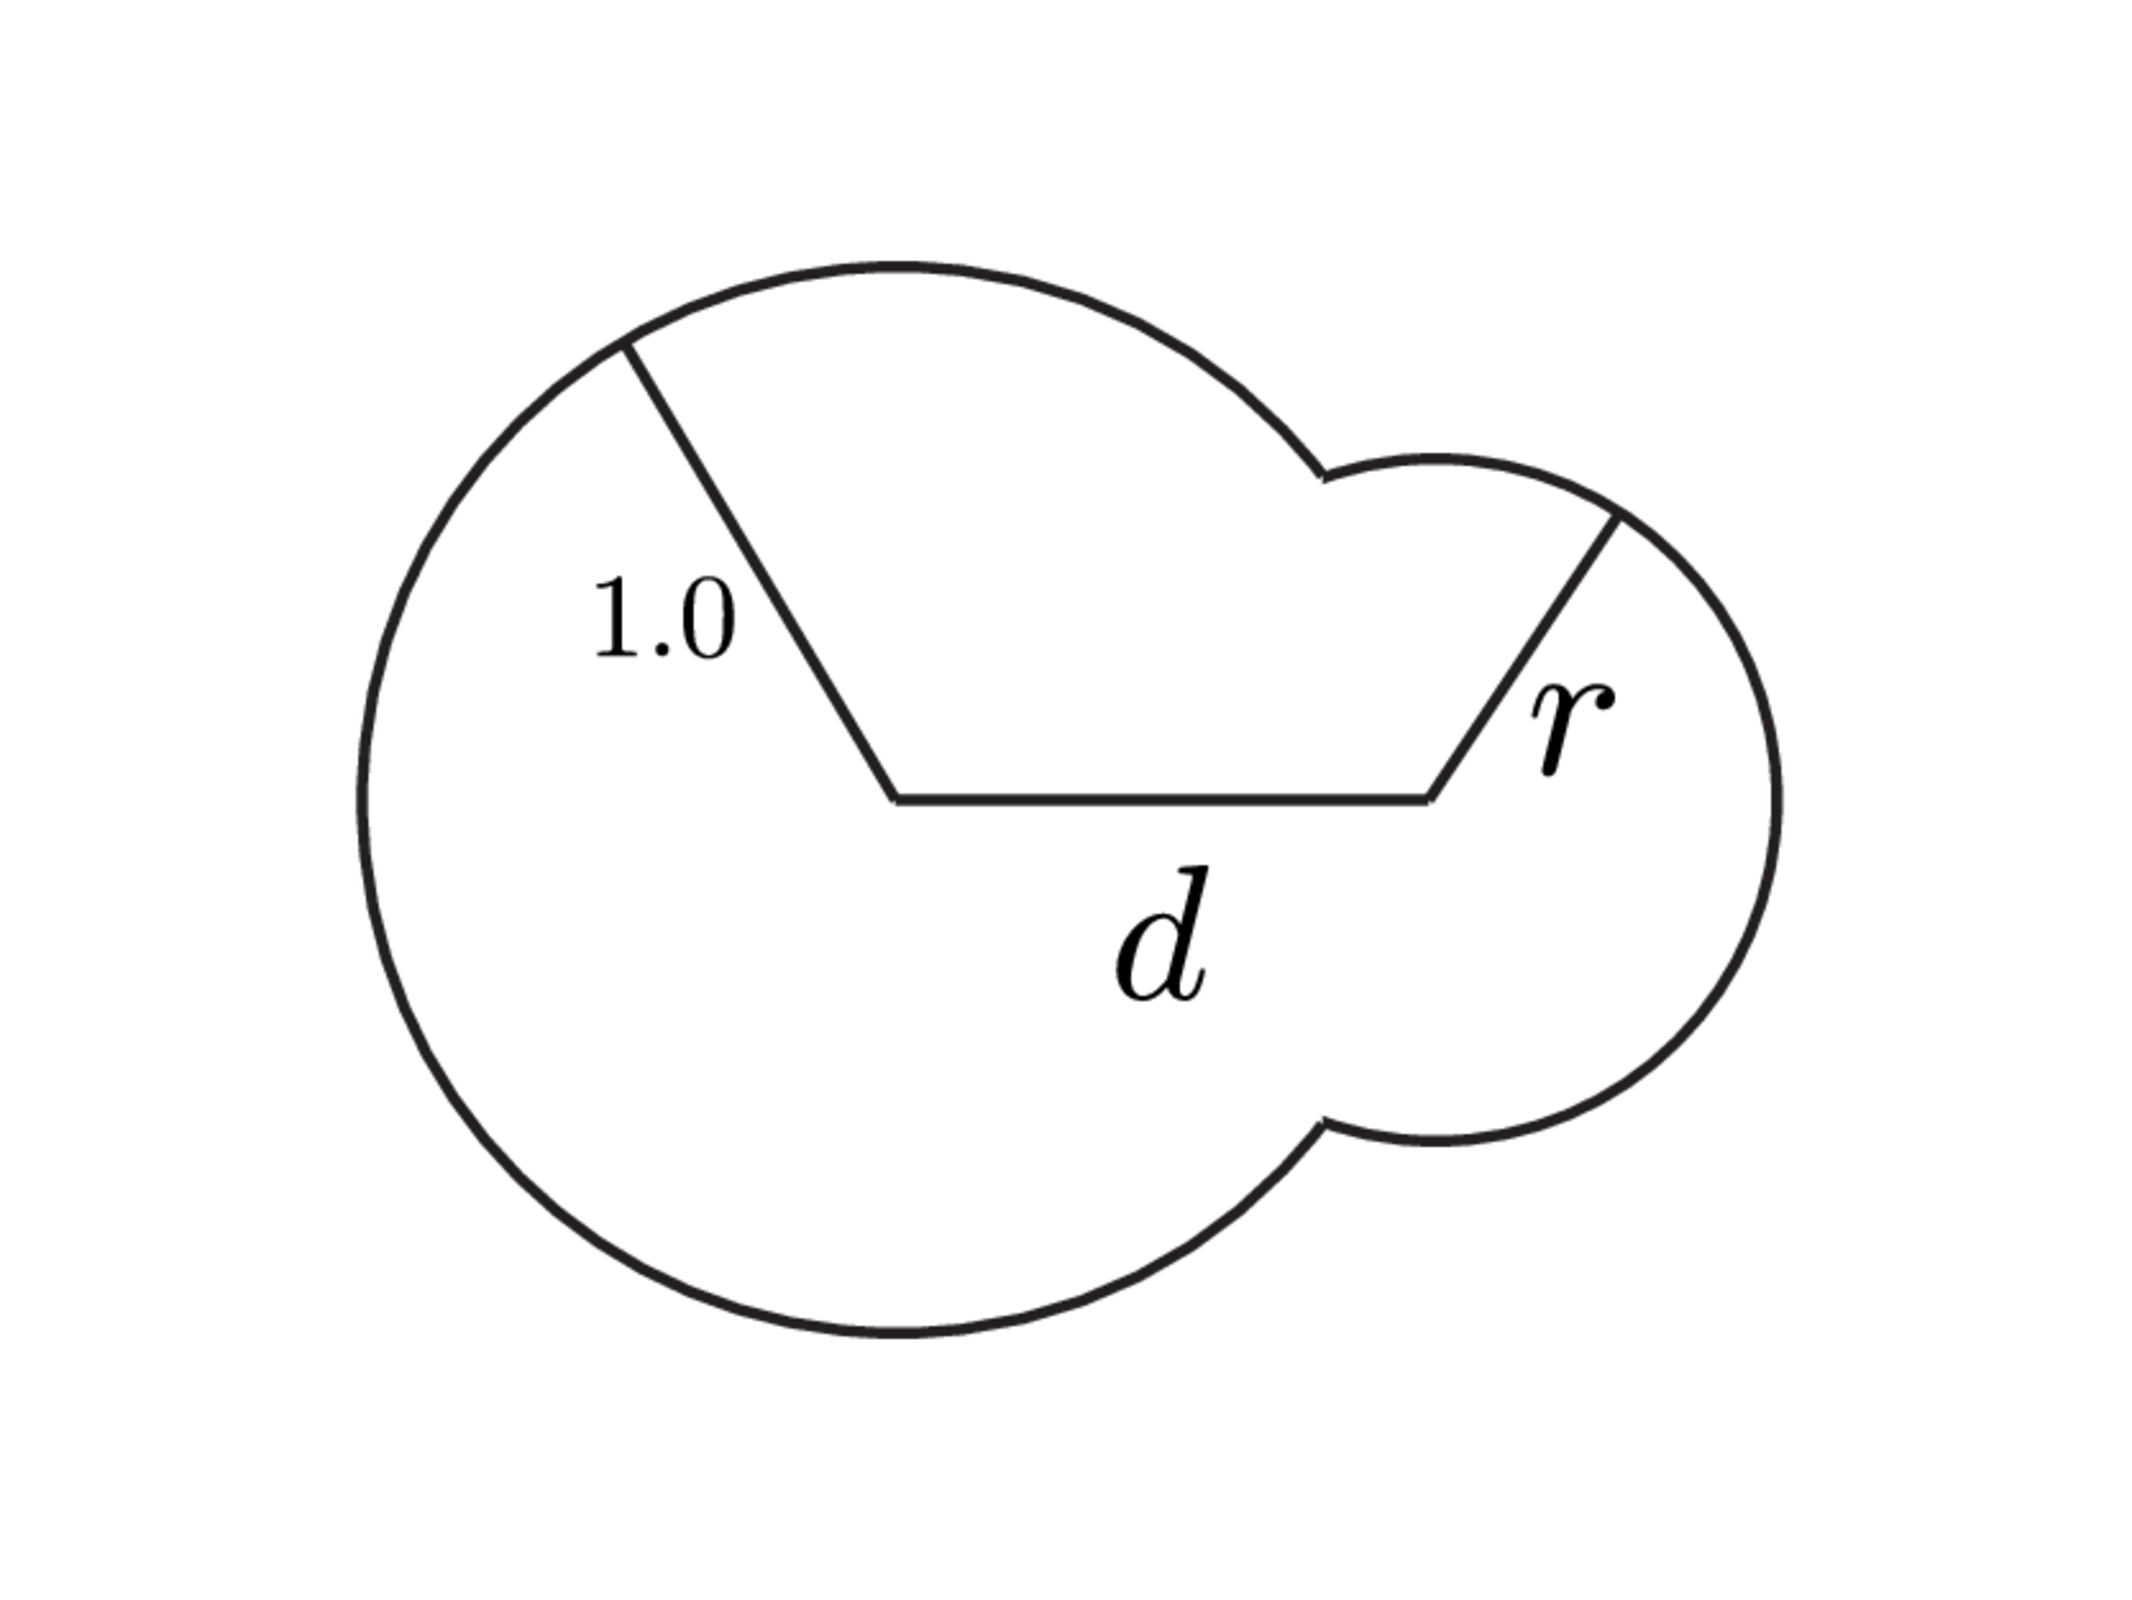
\includegraphics[width=\linewidth]{dimer}
        \caption{The Dimer molecule consists of a large particle of radius $1.0$, a small particle of radius $r$ separated by a distance $d$.}
        \label{fig:dimer}
    \end{subfigure}\hfill
    \begin{subfigure}[t]{0.48\textwidth}
        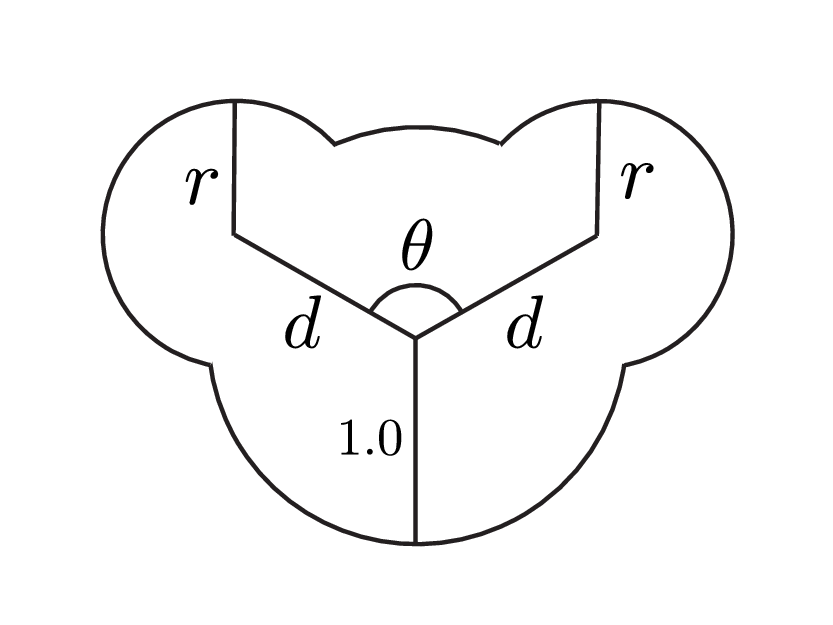
\includegraphics[width=\linewidth]{trimer}
        \caption{The Trimer molecule is comprised of a large particle of radius $1.0$ which subtends an angle $\theta$ between two small particles of radius $r$ at a distance $d$.}
        \label{fig:trimer}
    \end{subfigure}
    \caption{Construction of the molecules used in this thesis.}
    \label{fig:construction}
\end{figure}

The resulting collection of 50 molecules was cooled from a randomly generated high temperature state, resulting in a low temperature structure independent of the initial state. These low temperature structures were assessed for suitability on the criteria listed above, with one addition; the molecules chosen for in depth study had to be similar enough such that we could attribute any differences in dynamics to the shape of the molecule.

Hard discs with a radius $r=0.637556$ and $r=1.0$ have an interesting property, they can form an efficient binary packing of space, known as a compact packing~\appref{}. A dimer with a radius $r= 0.637556$ and a distance between the molecular centers $d= 1.637556$~\figref{dcon}, hereafter denoted \dcon has a crystal structure that mirrors this compact packing. Despite \dcon having a well defined crystal phase, the low temperature state exhibited none of this crystal, indicating a resilience to crystal formation. Retaining a radius of 0.637556 for the other molecules allows a more direct comparison, any differences between them are due to properties of the arrangement of particles, their shape, rather than the size ratios of the constituent particles. A distance $d= 1.0$ was chosen for another dimer~\figref{done} denoted \done and also for a trimer~\figref{tri} denoted \tri, for both consistency between the molecules and to allow all molecules to be described radially. An angle $\theta=120^\circ$ was chosen for the trimer as this angle allows the maximum number of interparticle interactions.

\begin{figure}
    \centering
    \captionsetup{justification=centering}
    \begin{subfigure}[t]{0.3\textwidth}
        \includegraphics[width=\linewidth]{{{Sone}}}
        \caption{\done}
        \label{fig:done}
    \end{subfigure}\hfill
    \begin{subfigure}[t]{0.3\textwidth}
        \includegraphics[width=\linewidth]{{{Scon}}}
        \caption{\dcon}
        \label{fig:dcon}
    \end{subfigure}\hfill
    \begin{subfigure}[t]{0.3\textwidth}
        \includegraphics[width=\linewidth]{{{Tri}}}
        \caption{\tri}
        \label{fig:tri}
    \end{subfigure}
    \caption{The molecules chosen for study in this thesis.}
    \label{fig:my mols}
\end{figure}

\section{Quantifying Dynamics in a Liquid}

There are three aspects of dynamics that we will measure in our liquids, translational motion, rotational motion and structural relaxation. Each of these aspects is directly related to an experimentally observable property, allowing the comparison of these results with those obtained in real world experiments.

For translational motion we shall determine the time dependence using the Mean Squared Displacement (MSD) of the centers of mass~\figref{msd ex}, given by
\begin{align}
    MSD(t) &= \langle \delta (t)^2 \rangle,\\
    \delta(t) &= \sqrt{(x(t) - x_0)^2 + (y(t) - y_0)^2}
    \label{eq:msd}
\end{align}
where $x(t)$ and $y(t)$ are the coordinates of the COM at time $t$, $x_0$ and $y_0$ are the initial coordinates of the molecule, and the angle brackets $\langle\,\rangle$ denote averaging over all molecules. For easier comparison we can find a characteristic value of the MSD, the diffusion constant $D$ is a measure of the rate of diffusion. The relationship between the MSD and the diffusion constant
\begin{equation}
    D = \frac{1}{4}\ddiff{\,MSD(t)}{t}
\end{equation} 
can be derived from the principles of Brownian motion~\tocite. The diffusion constant is the slope of the MSD at the long time limit, when the MSD is obeying a $t^1$ power law.

\begin{figure}
    \centering
    \includegraphics[width=0.5\textwidth]{{{msd}}}
    \caption{The mean squared displacement measures the distance the centers of mass ($\times$) move between the initial (grey) and final (black) positions.}
    \label{fig:msd ex}
\end{figure}

The second dynamic quantity we are interested in is the rotational relaxation, a measure of the rotational motions of the molecule~\figref{rot ex}. The \emph{rotational relaxation} $C_n(t)$ is given by
\begin{equation}
    C_n(t) = \langle P_n[\vect{\hat{e}}(0) \cdot \vect{\hat{e}}(t)] \rangle
    \label{eq:rot}
\end{equation}
where $P_n$ is the $n$\textsuperscript{th} order Legendre polynomial, $\vect{\hat{e}}(t)$ is the orientation vector at time $t$, and the angle brackets $\langle\,\rangle$ denote the averaging over all molecules. We are primarily interested in the first two rotational relaxation functions $C_1$ and $C_2$, in which the Legendre polynomials take the form
\begin{align}
    P_1(x) &= x\\
    P_2(x) &= 2x^2 - 1
\end{align}
as they have experimental analogues in dielectric relaxation, NMR, and optical methods~\cite{ediger:12}. The difference between the first order $C_1$ and second order $C_2$ relaxation functions is the angular size of the relaxations, $C_1$ is concerned with large angular motions and $C_2$ with smaller motions. The shape of both rotational relaxation functions is of exponential decay, making the \emph{rotational relaxation time} $\tau_n$, defined as the time for the rotational relaxation $C_n$ to reach a value of $1/\e$ an appropriate representation. In using this relaxation time as the characteristic value of the rotational relaxation function we are assuming the curve $\e^{-t/\tau_n}$ is a reasonable fit.

meaning an appropriate representative value of these functions is the time it takes to reach $1/\e$. Using this definition we can define a rotational relaxation time $\tau_n$ such that the curve $\e^{-t/\tau_n}$ is a good representation of the behaviour of the relaxation. 

\begin{figure}
    \centering
    \includegraphics[width=0.5\textwidth]{{{rot}}}
    \caption{The rotational relaxation is a measure of how much molecules have rotated (black) from their initial position (grey) taking the dot product of the orientation vectors of each molecule.}
    \label{fig:rot ex}
\end{figure}

In an real world system inelastic neutron scattering represents the most detailed account of relaxation in a liquid, combining information about the density fluctuations over a range of different length scales~\cite{perera:99}. The time correlation function associated with inelastic neutron scattering is the \emph{self-intermediate scattering function}~\tocite, defined as
\begin{equation}
    F_{S}(k,t) = \left \langle\e^{i\vect{k} \cdot [\vect r(t)-\vect r(0)]}\right \rangle
\end{equation}
where $\vect k$ is the wave vector, the magnitude of which is the magnitude of the density fluctuations, $\vect r(t)$ is the position at time $t$, and the angle brakets $\langle\,\rangle$ denote the averaging over all molecules and an angular average over the direction of the wave vector $\vect k$. A computationally simpler function that measures these same density relaxations is the \emph{structural relaxation function} and is defined by
\begin{align}
    F_d(t) = \left \langle \begin{cases}
        \quad0 &\text{if}\quad \delta > d \\
        \quad1 &\text{if}\quad \delta \leq d
    \end{cases} \quad \right \rangle
    \label{eq:struct}
\end{align}
where $d$ is the magnitude of the fluctuation, $\delta$ is the fluctuation from the initial position~\eqref{msd}, and the angle brackets denote averaging over all molecules~\cite{widmer:12}.

For our molecular liquids we shall define an analogue of the structural relaxation function~\eqref{struct} defined in terms of each individual particle. Specifically we find the structural relaxation function of each \emph{particle} and average over the total number of particles, giving the fraction of particles that remain with the threshold distance $d$ at time $t$~\figref{stuct ex}. We will use a threshold value of \num{0.3}, a value small enough for both translational and rotational motion of a molecule to contribute to the structural relaxation. As a way of a characteristic value of the structural relaxation we will be treating it in the same way as the rotational relaxation functions since the structural relaxation also undergoes an exponential relaxation. We define the structural relaxation time $\tau_s$ as the time for the structural relaxation function to reach a value of $1/\e$.

\begin{figure}
    \centering
    \includegraphics[width=0.5\textwidth]{{{struct}}}
    \caption{The structure function is a measure of how many particles have moved significantly from their initial positions (grey) with the threshold shown with a dotted green circle. Both rotational motion (depicted) and translational motion will result in particles moving out of this threshold region.}
    \label{fig:struct ex}
\end{figure} 

\section{Relaxation Dynamics of the Model Molecules; \done, \dcon and \tri}

In this Section we will be presenting the relaxation dynamics of each molecule over a range of temperatures. The temperature range reflects the temperatures over which the dynamics of each individual molecule are sufficiently fast to allow relaxation within a reasonable time. The simulations were monitored for signs of crystallisation and those temperature which showed crystal growth were discarded to ensure the relaxation dynamics measured are a property of the liquid phase.

The mean squared displacements~\figref{msd} of each molecule all show a similar features. At short times (\numrange{e-3}{e-1}) the MSD is in the ballistic regime characterised by a $t^2$ power law. The ballistic regime is where molecules are moving away from their initial position at constant velocity before they have collided with other molecules. At long times (\numrange{e5}{e7}) we have the diffusive regime characterised by a $t^1$ power law. The diffusive regime is where molecules have escaped their local environments and are undergoing random motion. At high temperatures ($\geq 2.50$) there is a direct transition from the ballistic regime to the diffusive regime, however at lower temperatures this transition is interrupted by a plateau region. The plateau region is where the molecules remain caged in their local environments and are unable to diffuse. As we decrease the temperature the plateau region extends in duration.

\begin{figure}
    \centering
    \begin{subfigure}[t]{\linewidth}
        \centering
        \includegraphics[width=0.7\textwidth]{{{Snowman-0.637556-1.0-msd}}}
        \caption{\done}
        \label{fig:done msd}
    \end{subfigure}
    \begin{subfigure}[t]{\linewidth}
        \centering
        \includegraphics[width=0.7\textwidth]{{{Snowman-0.637556-1.637556-msd}}}
        \caption{\dcon}
        \label{fig:dcon msd}
    \end{subfigure}
    \begin{subfigure}[t]{\linewidth}
        \centering
        \includegraphics[width=0.7\textwidth]{{{Trimer-0.637556-1.00-120-msd}}}
        \caption{\tri}
        \label{fig:tri msd}
    \end{subfigure}\hfill
    \caption{The Mean Squared Displacement, a measure a translational motion of the \done \subfigref{done msd}, \dcon \subfigref{dcon msd}, and \tri \subfigref{tri msd} molecules. The grey line indicates the $t^1$ power law defining the diffusive regime.}
    \label{fig:msd}
\end{figure}

The rotational relaxations~\figref{c1} of each molecule all show similar features. At high temperatures ($\geq 2.50$) we see exponential relaxation for all molecules. As we move to lower temperatures there is a deviation from this single exponential relaxation, we see a small initial relaxation to a plateau region, followed by an exponential relaxation. This two step relaxation process is similar to what we observe in the MSD, at low temperatures the relaxation is constrained by the local cage of molecules with relaxation occurring once escaped from the cage.

\begin{figure}
    \centering
    \begin{subfigure}[t]{\linewidth}
        \centering
        \includegraphics[width=0.7\textwidth]{{{Snowman-0.637556-1.0-C_1}}}
        \caption{\done}
        \label{fig:done c1}
    \end{subfigure}
    \begin{subfigure}[t]{\linewidth}
        \centering
        \includegraphics[width=0.7\textwidth]{{{Snowman-0.637556-1.637556-C_1}}}
        \caption{\dcon}
        \label{fig:dcon c1}
    \end{subfigure}
    \begin{subfigure}[t]{\linewidth}
        \centering
        \includegraphics[width=0.7\textwidth]{{{Trimer-0.637556-1.00-120-C_1}}}
        \caption{\tri}
        \label{fig:tri c1}
    \end{subfigure}\hfill
    \caption{The rotational relaxation function $C_1$, a measure of rotational motion for the \done \subfigref{done c1}, \dcon \subfigref{dcon c1}, and \tri \subfigref{tri c1} molecules.}
    \label{fig:c1}
\end{figure}

The structural relaxations~\figref{F}, exhibit some interesting features. At short timescales (\numrange{e-3}{e-1}) the molecules have not had enough time to move the required distance for structural relaxation. At high temperatures ($\geq 2.50$) we then see a sharp dropoff, characteristic of the step function used, to an exponential relaxation. However at low temperatures we begin to see a region with oscillations most obvious in the \tri molecule~\figref{tri F}. These oscillations are a result of entire system vibrations collectively moving particles~\cite{perera:99}. This oscillatory region is similar to the plateau region in the rotational relaxation in that it is the transition region between the two steps of a two step relaxation process. In the structural relaxation function this second relaxation no longer has an exponential shape, indicating a more complicated relaxation process.

\begin{figure}
    \begin{subfigure}[t]{\linewidth}
        \centering
        \includegraphics[width=0.7\textwidth]{{{Snowman-0.637556-1.0-F}}}
        \caption{\done}
        \label{fig:done F}
    \end{subfigure}
    \begin{subfigure}[t]{\linewidth}
        \centering
        \includegraphics[width=0.7\textwidth]{{{Snowman-0.637556-1.637556-F}}}
        \caption{\dcon}
        \label{fig:dcon F}
    \end{subfigure}
    \begin{subfigure}[t]{\linewidth}
        \centering
        \includegraphics[width=0.7\textwidth]{{{Trimer-0.637556-1.00-120-F}}}
        \caption{\tri}
        \label{fig:tri F}
    \end{subfigure}\hfill
    \caption{The structural relaxation function $F$ for the \done \subfigref{done F}, \dcon \subfigref{dcon F}, and \tri \subfigref{tri F} molecules. The oscillations, most noticable in \subfigref{tri F} show the effects of system wide vibrations.}
    \label{fig:F}
\end{figure}

Comparing the dynamic quantities of the three molecules~\figref{dynamic comparison} using the characteristic values of the dynamic quantities there are large differences between the molecules. Looking at the diffusion constant~\figref{D}, \done shows a close to linear decrease in the diffusion constant as the temperature decreases. This linear behaviour is consistent with the Arrhenius relation and indicates that these molecular rearrangements have a constant activation energy. The \dcon molecule shows definite non-Arrhenius behaviour, with the diffusion constant diverging from that of \done by more than three orders of magnitude despite comparable values at high temperatures. The \tri molecule tracks between the \done and \dcon molecules. Both the rotational relaxation~\figref{t1} and structural relaxation~\figref{ts} show similar behaviour to the diffusion constant, \done shows linear temperature dependence, the behaviour of a strong glass forming liquid. The \dcon molecule exhibits a significant increase as the temperature decreases, the behaviour of a fragile liquid. The final molecule, \tri sits between the \done and the \dcon molecules covering the range of dynamic behaviour of supercooled liquids.

The structural relaxation~\figref{ts} displays two gradients for each of the molecules, indicative of two separate relaxation processes with different activation energies. At high temperatures there is a process with a low activation energy (small gradient) which suddenly transitions at lower temperatures, to a process with a high activation energy (large gradient). Neither the diffusion constant or the rotational relaxation show this sudden transition between two processes. By taking the relative contributions of the diffusion constant and the rotational relaxation time to the structural relaxation time\figref{ts cont}, the change in relaxation process is clearly seen as the inflection point. Initially the structural relaxation is dominated by translational motion, a process with a low activation energy. However at the inflection point the process changes to one dominated by rotational motion with at higher activation energy. Further evidence of this transition comes from comparing the activation energies of the rotational~\figref{t1} and structural~\figref{ts} relaxations, after the transition of the structural relaxation to a rotationally dominated process the activation energies show strong correlations. Despite the sudden change in the dynamics of the structural relaxation, there is no corresponding discontinuity in the diffusion constant~\figref{D}. This is due to the definition of the diffusion constant, we are only interested in the gradient of the MSD in the diffusive regime, ignoring the time to reach the diffusive regime. At low temperatures the plateau region of the MSD is sits below the 0.09 cutoff of the structure function, during which rotations are the primary contributor to the structural relaxation. 

\begin{figure}
    \centering
    \begin{subfigure}{\linewidth}
        \centering
        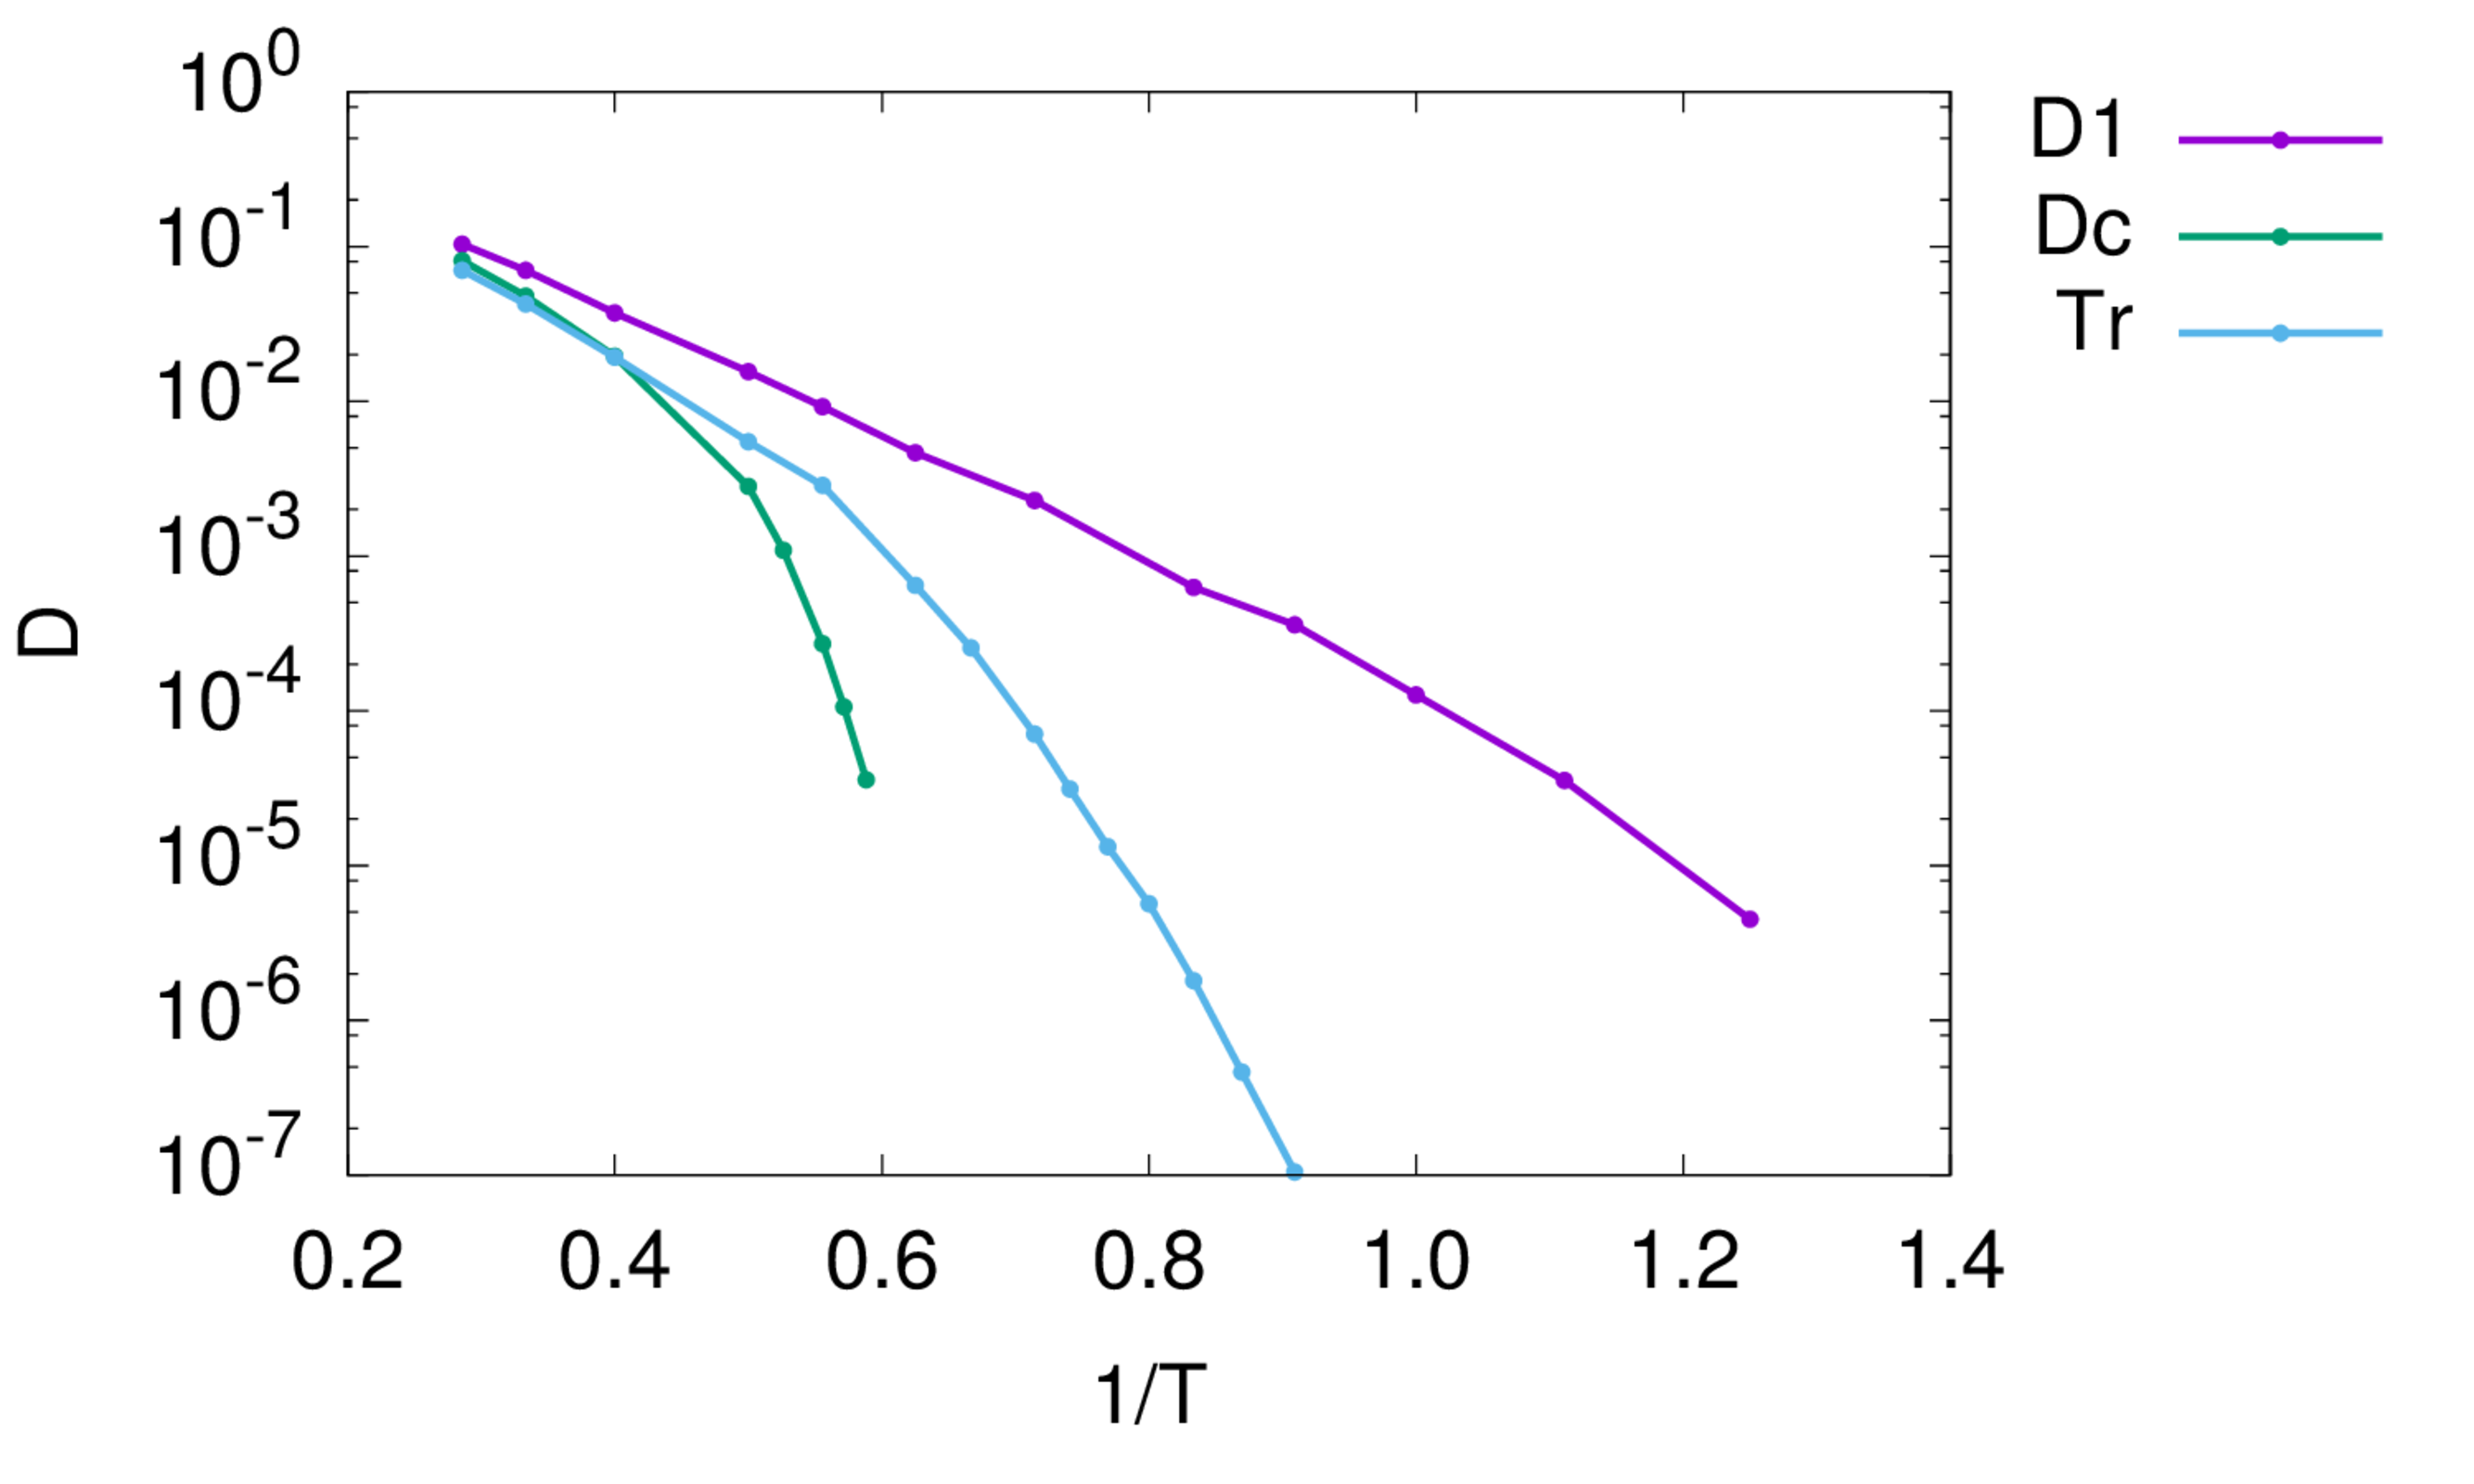
\includegraphics[width=0.6\textwidth]{D}
        \caption{}
        \label{fig:D}
    \end{subfigure}
    \begin{subfigure}{\linewidth}
        \centering
        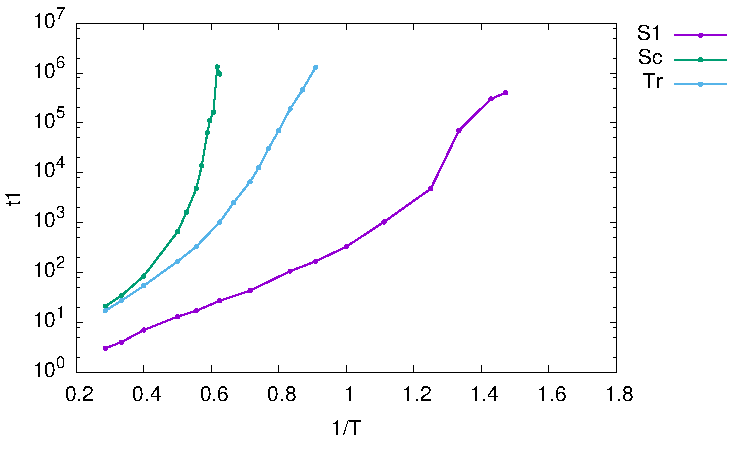
\includegraphics[width=0.6\textwidth]{t1}
        \caption{}
        \label{fig:t1}
    \end{subfigure}
    \begin{subfigure}{\textwidth}
        \centering
        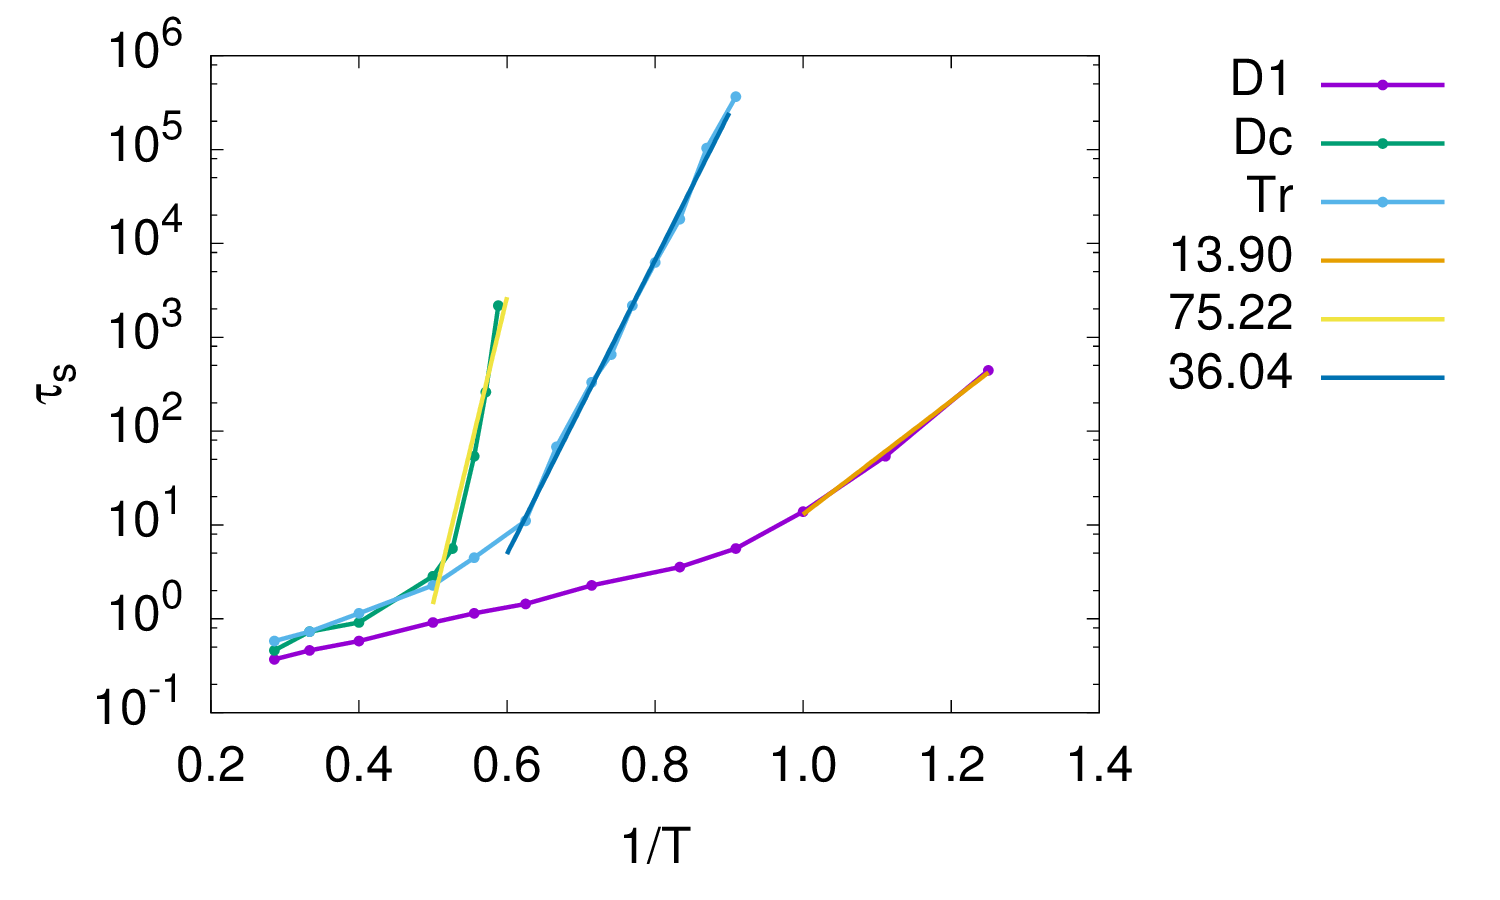
\includegraphics[width=0.6\textwidth]{ts}
        \caption{}
        \label{fig:ts}
    \end{subfigure}
    \caption{Comparison of the diffusion constant~\subfigref{D}, rotational relaxation time $\tau_1$~\subfigref{t1}, and structural relaxation time $\tau_s$~\subfigref{ts} for the three molecules that we are studying. As we move from \done to \tri to \dcon the dynamics of the liquid become increasingly non-Arrhenius. The activation energy of the rotational relaxation \subfigref{t1} and the structural relaxation \subfigref{ts} are found from the gradients of the functions as plotted.}
    \label{fig:dynamic comparison}
\end{figure}

\begin{figure}
    \begin{subfigure}{0.5\textwidth}
        \includegraphics[width=\textwidth]{{{D.ts}}}
        \caption{}
        \label{fig:d.ts}
    \end{subfigure}
    \begin{subfigure}{0.5\textwidth}
        \includegraphics[width=\textwidth]{{{t1.ts}}}
        \caption{}
        \label{fig:t1.ts}
    \end{subfigure}
    \caption{Relative contribution of diffusion \subfigref{d.ts} and rotation \subfigref{t1.ts} to structural relaxation over a number of temperatures. The discontinuity shows the point at which the structural relaxation moves from being dominated by translational motion to being dominated by rotational motion.}
    \label{fig:ts cont}
\end{figure}


\section{Analysis of the Coupling of Diffusion and Rotation}

The increased contribution of the rotations to the overall dynamics is an interesting result, previous studies both experimental~\cite{stillinger:94,cicerone:95,debenedetti:01,swallen:03} and simulated~\cite{kammerer:97} have found that translations, rather than rotations dominate the rearrangements at low temperatures contrary to our observations of the structural relaxation. 

Along with dominating the structural relaxation, the dominance of rotations in our systems is also seen when taking the product of the diffusion constant and the rotational relaxation~\figref{D.t1}, the diffusion constant is getting smaller faster than the rotational relaxation time is increasing. One possible explanation for the dominance of rotations over translations in our molecules at low temperature is that when molecules interlock via a concavity the concavity inhibits the translational motion, molecules have to unlock from the concavity to move past one another. Rotations however, are still possible while retaining the interaction at the concavity.

\begin{figure}
    \centering
    \includegraphics[width=0.6\textwidth]{{{D.t1}}}
    \caption{Relative contributions of the diffusion constant and rotational relaxation to the overall dynamics. The decrease of this product as the temperature decreases indicates the translational diffusion is getting slower faster than the rotational relaxation increases.}
    \label{fig:D.t1}
\end{figure}

Studying the rotations of our molecules further, results of simulations using similar molecules~\cite{kammerer:97,michele:01} found that at low temperatures molecules underwent rotational relaxation by flips of \ang{180}. To investigate the contribution of \ang{180} jumps in our molecules we can compare the first and second order rotational relaxation times, since flips of \ang{180} do not contribute to the second order relaxation. Taking the ratio of the first and second relaxation times $\tau_1/\tau_2$~\figref{t1/t2}, we see a decrease in this ratio for all molecules, $\tau_2$ is larger than $\tau_1$ at low temperature meaning there is little contribution to the relaxation be \ang{180} flips in orientation.

\begin{figure}
    \centering
    \includegraphics[width=0.6\textwidth]{{{t1.t2}}}
    \caption{The ratio of the first and second order rotational relaxation times as a function of temperature. As the temperature decreases the decrease in this ratio shows that molecules undergo small angle changes rather than large \ang{180} flips.}
    \label{fig:t1/t2}
\end{figure}

In describing the differences between the dynamic properties of the molecules the Aperiodic Crystal Structure model provides a relationship between the rotational relaxation and the diffusion constant, and the local structural rigidity in the Hall-Wolynes equation~\cite{hall:87,dyre:96}
\begin{equation}
    \tau_1, D \propto \e^{a^2/2\langle u^2\rangle}
\end{equation}
where $a$ is the displacement to overcome the local energy barrier and $\langle u^2 \rangle$ is the Debye-Waller factor, a measure of the local rigidity of the structure. The Debye-Waller factor is found as the MSD at the time where 
\begin{equation}
    \ddiff{\log{(\text{MSD})}}{\log{(t)}}
\end{equation}
is a minimised~\cite{larini:08}, the value where the slope is lowest in \textfigref{msd}. The Debye-Waller factor of our molecules is shown in \textfigref{DW}, there is an initial high temperature region where the Debye-Waller factor is constant, followed by an exponential decrease. The Debye-Waller factors of the \dcon and \tri are remarkably similar over a large portion of the temperature range.

Plotting the diffusion constant~\figref{DW.D} and the rotational relaxation time~\figref{DW.t1} against $1/\langle u^2 \rangle$ we see that instead of the behaviour of the molecules diverging there is a strong correlation. The Debye-Waller factor normalises the dynamics on the local structural rigidity explaining a significant portion of the difference in the dynamics of the molecules. In changing the shape of molecules we change the local stiffness of the liquid phase resulting in order of magnitude changes of the dynamics. The cause of the temperature dependence of the local stiffness is likely a key contributor to the fragility of a liquid.

\begin{figure}
    \centering
    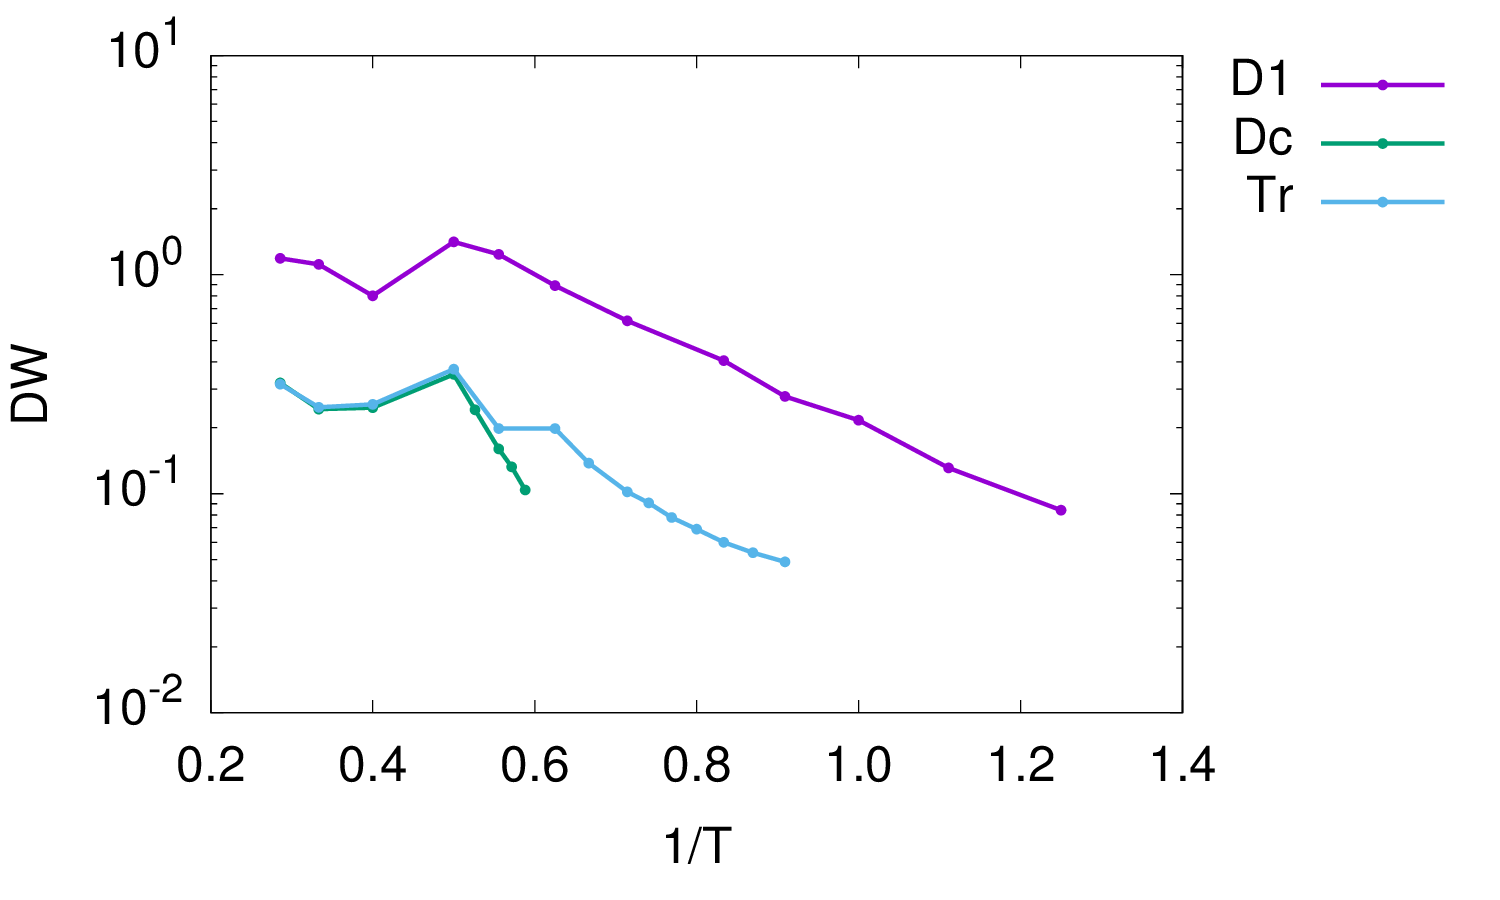
\includegraphics[width=0.6\textwidth]{DW}
    \caption{The temperature dependence of the Debye-Waller factor for each molecule. At high temperatures the Debye-Waller factor is relatively constant before an exponential decrease.}
    \label{fig:DW}
\end{figure}

\begin{figure}
    \centering
    \begin{subfigure}{0.6\textwidth}
        \includegraphics[width=\textwidth]{{{DW.D}}}
        \caption{}
        \label{fig:DW.D}
    \end{subfigure}
    \begin{subfigure}{0.6\textwidth}
        \includegraphics[width=\textwidth]{{{DW.t1}}}
        \caption{}
        \label{fig:DW.t1}
    \end{subfigure}
    \caption{By normalising the diffusion constant~\subfigref{DW.D} and rotational relaxation~\subfigref{DW.t1} by the Debye-Waller factor we are able to account for significant differences in the dynamic quantities. At high temperatures the Debye-Waller factor $\langle u^2 \rangle$ is a fairly constant large value (left of figure). As the temperature decreases both \done and \tri show similar rotational relaxation times. The \dcon molecule shows a steeper slope indicating the presence of more complicated process.}
\end{figure}

\section{Summary}

In this Chapter we have found that small changes to molecular shape play an important role in the dynamics of the liquid phase, resulting in relaxation times that differ by up to four orders of magnitude. Much of these differences in dynamics can be explained by the local structural rigidity. It is molecular structure and how it is influenced molecular shape that we investigate in the following Chapter.

